% example-3-narrative.tex
% Self-contained extract from example.tex (compile: pdflatex example-3-narrative.tex, run twice).

\documentclass[11pt]{article}

\usepackage[margin=1in]{geometry}
\usepackage{amsmath}
\usepackage{enumitem}
\usepackage{xcolor}
\usepackage{soul}
\usepackage{tikz}
\usetikzlibrary{arrows.meta,positioning,calc,backgrounds}

% --- atomic-unit highlight palette ---
\definecolor{cP1}{RGB}{210,228,248}
\definecolor{cP2}{RGB}{252,243,207}
\definecolor{cP3}{RGB}{215,236,219}
\definecolor{cP4}{RGB}{226,221,243}
\definecolor{cP5}{RGB}{249,222,229}
\definecolor{cP6}{RGB}{222,240,243}
\definecolor{cPivot}{RGB}{250,219,180}   % pivotal revelation

% \fu{colour}{span}{label}: highlight a clause and tag it with its atomic-unit id.
% \hl (soul) wraps across line breaks.
\sethlcolor{cP1}
\newcommand{\fu}[3]{{\sethlcolor{#1}\hl{#2}}\,\textsuperscript{\textbf{\scriptsize #3}}}

\title{Example 3: A Narrative Passage (Elinor)}
\author{FactReasoner --- Ideation}
\date{\today}

\begin{document}
\maketitle
\section{A narrative passage (Elinor)}

\subsection*{Source paragraph}

\noindent\textbf{Plain text.}
\begin{quote}
Elinor is surprised no letter arrives with details about the marriage, and she
wonders how Edward felt being close to Barton. Elinor asks her mother to write to
Colonel Brandon for news, realizing she hoped something would prevent Edward's
marriage. Elinor feels incredibly hurt by Edward's marriage. Colonel Brandon
arrives at the house, but it is revealed to be Edward instead. Elinor is surprised
that Edward and Lucy were married so soon, and she mulls over the event of
Edward's marriage, supposing that the Ferrars must be settled at Delaford,
envisioning Edward and Lucy's life there. Edward enters the room looking ill with
anxiety, and Elinor tells herself to be calm upon Edward's arrival. Elinor thinks
someone in London might have informed her about Edward and Lucy's marriage.
Marianne and Margaret retreat, leaving Elinor and Mrs.~Dashwood with Edward,
while Marianne and Mrs.~Dashwood react with shock and uncertainty about Edward's
arrival. Mrs.~Dashwood breaks the ice by shaking Edward's hand and wishing him
happiness. However, no word has arrived from Colonel Brandon, and Mrs.~Dashwood
asks about Mrs.~Ferrars' health, to which Elinor inquires if Mrs.~Ferrars is at
Longstaple. Edward is shocked to discover his mother is not nearby, and Elinor
pointedly asks about Mrs.~Edward Ferrars. Edward is confused and asks if Elinor
means Mrs.~Robert Ferrars instead, leading to everyone being shocked by the
revelation that Robert married Lucy Steele. Elinor flees the room, unsure of how
to react, and bursts into tears of joy. Edward sits in silence, unsure of what to
do, then simply leaves the room. Everyone is left perplexed by the situation.
\end{quote}

\noindent\textbf{Annotated.} Each highlighted clause is one atomic unit
\textsuperscript{\textbf{\scriptsize F\textit{n}}}; the rotating colours just
separate adjacent units, and the pivotal revelation \textbf{F27} is orange.

\begin{quote}
\fu{cP1}{Elinor is surprised no letter arrives with details about the marriage}{F1}, and she
\fu{cP2}{wonders how Edward felt being close to Barton}{F2}.
\fu{cP3}{Elinor asks her mother to write to Colonel Brandon for news}{F3},
\fu{cP4}{realizing she hoped something would prevent Edward's marriage}{F4}.
\fu{cP5}{Elinor feels incredibly hurt by Edward's marriage}{F5}.
\fu{cP6}{Colonel Brandon arrives at the house}{F6}, but
\fu{cP1}{it is revealed to be Edward instead}{F7}.
\fu{cP2}{Elinor is surprised that Edward and Lucy were married so soon}{F8}, and she
\fu{cP3}{mulls over the event of Edward's marriage}{F9},
\fu{cP4}{supposing that the Ferrars must be settled at Delaford}{F10},
\fu{cP5}{envisioning Edward and Lucy's life there}{F11}.
\fu{cP6}{Edward enters the room looking ill with anxiety}{F12}, and
\fu{cP1}{Elinor tells herself to be calm upon Edward's arrival}{F13}.
\fu{cP2}{Elinor thinks someone in London might have informed her about Edward and Lucy's marriage}{F14}.
\fu{cP3}{Marianne and Margaret retreat}{F15},
\fu{cP4}{leaving Elinor and Mrs.~Dashwood with Edward}{F16}, while
\fu{cP5}{Marianne and Mrs.~Dashwood react with shock and uncertainty about Edward's arrival}{F17}.
\fu{cP6}{Mrs.~Dashwood breaks the ice by shaking Edward's hand}{F18} and
\fu{cP1}{wishing him happiness}{F19}. However,
\fu{cP2}{no word has arrived from Colonel Brandon}{F20}, and
\fu{cP3}{Mrs.~Dashwood asks about Mrs.~Ferrars' health}{F21}, to which
\fu{cP4}{Elinor inquires if Mrs.~Ferrars is at Longstaple}{F22}.
\fu{cP5}{Edward is shocked to discover his mother is not nearby}{F23}, and
\fu{cP6}{Elinor pointedly asks about Mrs.~Edward Ferrars}{F24}.
\fu{cP1}{Edward is confused}{F25} and
\fu{cP2}{asks if Elinor means Mrs.~Robert Ferrars instead}{F26}, leading to
\fu{cP3}{everyone being shocked}{F28} by the
\fu{cPivot}{revelation that Robert married Lucy Steele}{F27}.
\fu{cP5}{Elinor flees the room, unsure of how to react}{F29}, and
\fu{cP6}{bursts into tears of joy}{F30}.
\fu{cP1}{Edward sits in silence, unsure of what to do}{F31},
\fu{cP2}{then simply leaves the room}{F32}.
\fu{cP3}{Everyone is left perplexed by the situation}{F33}.
\end{quote}

\subsection*{Atomic units (self-contained, in order of appearance)}

Pronouns are resolved to their referents so each unit stands alone.

\begin{enumerate}[label=\textbf{F\arabic*.},leftmargin=*]
  \item Elinor is surprised that no letter arrives with details about the marriage.
  \item Elinor wonders how Edward felt being close to Barton.
  \item Elinor asks her mother to write to Colonel Brandon for news.
  \item Elinor realizes she had hoped something would prevent Edward's marriage.
  \item Elinor feels incredibly hurt by Edward's marriage.
  \item A visitor arrives at the house and is initially taken to be Colonel Brandon.
  \item The visitor is revealed to be Edward instead of Colonel Brandon.
  \item Elinor is surprised that Edward and Lucy were married so soon.
  \item Elinor mulls over the event of Edward's marriage.
  \item Elinor supposes that the Ferrars must be settled at Delaford.
  \item Elinor envisions Edward and Lucy's life at Delaford.
  \item Edward enters the room looking ill with anxiety.
  \item Elinor tells herself to be calm upon Edward's arrival.
  \item Elinor thinks someone in London might have informed her about Edward and Lucy's marriage.
  \item Marianne and Margaret retreat from the room.
  \item Marianne and Margaret leave Elinor and Mrs.~Dashwood alone with Edward.
  \item Marianne and Mrs.~Dashwood react with shock and uncertainty about Edward's arrival.
  \item Mrs.~Dashwood breaks the ice by shaking Edward's hand.
  \item Mrs.~Dashwood wishes Edward happiness.
  \item No word has arrived from Colonel Brandon.
  \item Mrs.~Dashwood asks about Mrs.~Ferrars' health.
  \item Elinor inquires whether Mrs.~Ferrars is at Longstaple.
  \item Edward is shocked to discover Edward's mother is not nearby.
  \item Elinor pointedly asks about Mrs.~Edward Ferrars.
  \item Edward is confused by Elinor's question about Mrs.~Edward Ferrars.
  \item Edward asks whether Elinor means Mrs.~Robert Ferrars instead.
  \item It is revealed that Robert married Lucy Steele.
  \item Everyone is shocked by the revelation that Robert married Lucy Steele.
  \item Elinor flees the room, unsure of how to react.
  \item Elinor bursts into tears of joy.
  \item Edward sits in silence, unsure of what to do.
  \item Edward then leaves the room.
  \item Everyone is left perplexed by the situation.
\end{enumerate}

\subsection*{Relations}

\textbf{Logical prerequisites ($A \rightarrow B$).} In a narrative the
prerequisite relation is largely \emph{enabling causation / temporal grounding}:
an earlier event makes a later one possible or meaningful.

\begin{itemize}[leftmargin=*]
  \item F6 $\rightarrow$ F7 --- a visitor must arrive before being re-identified as Edward.
  \item F7 $\rightarrow$ F12 --- Edward being the arrival is presupposed by Edward entering the room.
  \item F9 $\rightarrow$ F10 --- mulling over the marriage grounds the supposition about Delaford.
  \item F10 $\rightarrow$ F11 --- supposing the Ferrars settle at Delaford grounds envisioning their life there.
  \item F15 $\rightarrow$ F16 --- Marianne and Margaret must retreat for Elinor and Mrs.~Dashwood to be left with Edward.
  \item F22 $\rightarrow$ F23 --- Elinor's question about Longstaple prompts Edward's discovery his mother is not nearby.
  \item F24 $\rightarrow$ F25 --- the pointed question about ``Mrs.~Edward Ferrars'' is what confuses Edward.
  \item F25 $\rightarrow$ F26 --- Edward's confusion grounds his counter-question about Mrs.~Robert Ferrars.
  \item F26 $\rightarrow$ F27 --- Edward's counter-question surfaces the revelation that Robert married Lucy.
  \item F27 $\rightarrow$ F28 --- the revelation is what shocks everyone.
  \item F27 $\rightarrow$ F30 --- the revelation (Edward is \emph{not} married) is why Elinor's tears are tears of \emph{joy}.
\end{itemize}

\noindent
\textbf{Position invalidations ($A \neq B$).} The pivotal unit is \textbf{F27}:
the revelation that it was \emph{Robert} (not Edward) who married Lucy Steele.
Appearing late in the passage, it retroactively invalidates the false premise --
woven through the entire opening -- that \emph{Edward} married Lucy.

\begin{itemize}[leftmargin=*]
  \item F27 $\neq$ F1 --- the awaited ``marriage'' news concerned a marriage of Edward that never happened.
  \item F27 $\neq$ F4 --- there was no marriage of Edward for Elinor to have hoped to prevent.
  \item F27 $\neq$ F5 --- Elinor's hurt rested on a marriage of Edward that did not occur.
  \item F27 $\neq$ F8 --- ``Edward and Lucy were married so soon'' is false; Edward did not marry Lucy.
  \item F27 $\neq$ F9 --- there was no ``event of Edward's marriage'' to mull over.
  \item F27 $\neq$ F10 --- the Ferrars settling at Delaford as a married couple (Edward + Lucy) is invalidated.
  \item F27 $\neq$ F11 --- the envisioned life of Edward and Lucy at Delaford never existed.
  \item F27 $\neq$ F14 --- the supposed London report of \emph{Edward and Lucy's} marriage was mistaken.
\end{itemize}

\noindent
\textbf{Note.} The invalidations all share a single source (F27) and a single
target premise (``Edward married Lucy''). The events of arrival, greeting, and
dialogue (F6, F7, F12--F26) are \emph{not} invalidated -- they actually happened;
only Elinor's (and the narrator's) interpretation of \emph{who} was married is
overturned.

\subsection*{Relation graph}

Solid blue arrows are logical prerequisites ($A \rightarrow B$). Dashed red
arrows are position invalidations ($A \neq B$), all emanating from the pivotal
revelation \textbf{F27}. The eight invalidated ``Edward-married-Lucy'' premises
are tinted red; F27 is highlighted.

\begin{center}
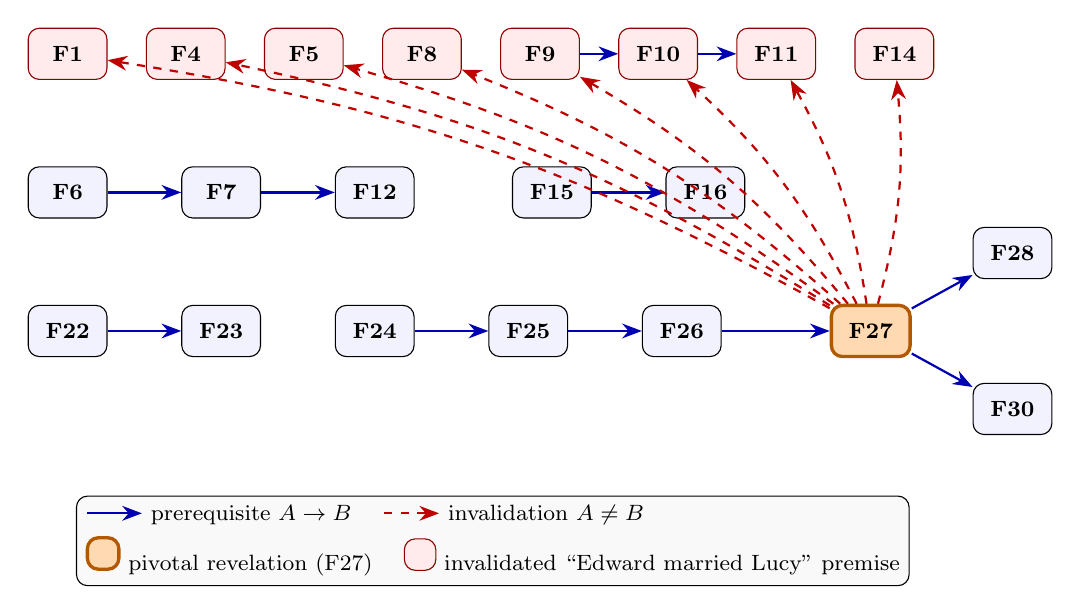
\begin{tikzpicture}[
    >={Stealth[length=2.5mm]},
    x=15mm, y=11mm,
    nnode/.style={draw,rounded corners,minimum width=10mm,minimum height=6.5mm,
                  inner sep=1pt,font=\footnotesize\bfseries,fill=blue!5},
    pivot/.style={nnode,fill=orange!30,draw=orange!70!black,very thick},
    falsey/.style={nnode,fill=red!8,draw=red!55!black},
    prereq/.style={->,blue!70!black,thick},
    invalid/.style={->,red!75!black,dashed,thick},
  ]

  % Layout: invalidated premises along the TOP row (the false "Edward married
  % Lucy" thread), the live event chain along the MIDDLE/BOTTOM, F27 at the
  % pivot on the right. Generous, uniform spacing prevents any overlap.

  % --- top row: the invalidated premises (tinted red) ---
  \node[falsey] (f1)  at (0,4)  {F1};
  \node[falsey] (f4)  at (1,4)  {F4};
  \node[falsey] (f5)  at (2,4)  {F5};
  \node[falsey] (f8)  at (3,4)  {F8};
  \node[falsey] (f9)  at (4,4)  {F9};
  \node[falsey] (f10) at (5,4)  {F10};
  \node[falsey] (f11) at (6,4)  {F11};
  \node[falsey] (f14) at (7,4)  {F14};

  % --- supposition chain (just below the top row, left) ---
  \draw[prereq] (f9)  -- (f10);
  \draw[prereq] (f10) -- (f11);

  % --- arrival sub-chain (upper-middle, left) ---
  \node[nnode] (f6)  at (0,2.4) {F6};
  \node[nnode] (f7)  at (1.3,2.4) {F7};
  \node[nnode] (f12) at (2.6,2.4) {F12};
  \draw[prereq] (f6) -- (f7);
  \draw[prereq] (f7) -- (f12);

  % --- retreat ---
  \node[nnode] (f15) at (4.1,2.4) {F15};
  \node[nnode] (f16) at (5.4,2.4) {F16};
  \draw[prereq] (f15) -- (f16);

  % --- dialogue / discovery chain (middle row) ---
  \node[nnode] (f22) at (0,0.8)   {F22};
  \node[nnode] (f23) at (1.3,0.8) {F23};
  \node[nnode] (f24) at (2.6,0.8) {F24};
  \node[nnode] (f25) at (3.9,0.8) {F25};
  \node[nnode] (f26) at (5.2,0.8) {F26};
  \draw[prereq] (f22) -- (f23);
  \draw[prereq] (f24) -- (f25);
  \draw[prereq] (f25) -- (f26);

  % --- the pivot and its consequences (bottom-right) ---
  \node[pivot] (f27) at (6.8,0.8)  {F27};
  \node[nnode] (f28) at (8.0,1.7)  {F28};
  \node[nnode] (f30) at (8.0,-0.1) {F30};
  \draw[prereq] (f26) -- (f27);
  \draw[prereq] (f27) -- (f28);
  \draw[prereq] (f27) -- (f30);

  % --- invalidation edges: F27 fans up to each false premise on the top row.
  %     A gentle uniform rightward bend keeps the eight dashed edges parallel
  %     and clear of the node labels. ---
  \foreach \t in {f1,f4,f5,f8,f9,f10,f11,f14} {
    \draw[invalid] (f27) to[bend right=10] (\t);
  }

  % --- legend ---
  \node[draw,fill=gray!5,rounded corners,anchor=north,align=left,
        font=\footnotesize] at (3.6,-1.1) {
    \tikz\draw[prereq](0,0)--(7mm,0);~prerequisite $A\rightarrow B$
    \quad
    \tikz\draw[invalid](0,0)--(7mm,0);~invalidation $A\neq B$\\[3pt]
    \tikz\node[pivot,minimum width=4mm,minimum height=4mm]{};~pivotal revelation (F27)
    \quad
    \tikz\node[falsey,minimum width=4mm,minimum height=4mm]{};~invalidated ``Edward married Lucy'' premise
  };

\end{tikzpicture}
\end{center}

\noindent\emph{(For legibility the graph shows the principal chains and the full
invalidation fan; purely sequential narration edges such as F1--F2 or F31--F32
are omitted. The mapping of these units onto the ground-truth scene below is
given in Table~\ref{tab:gt-align}, and the ground-truth dependency graph in
Figure~\ref{fig:gt-graph}.)}

\subsection*{Comparison against the ground-truth passage}

The paragraph analysed above is a paraphrase of the following \emph{ground-truth}
account of the same scene. We re-decompose the ground truth, align it to the
units F1--F33, and check that the relation structure (the pivot at the
``Robert married Lucy'' revelation, and the invalidation fan it triggers) is
preserved.

\noindent\textbf{Plain text.}
\begin{quote}
Elinor finds herself mulling over the event of Edward's marriage --- she realizes
that she'd hoped that something would come up to prevent it, but now that it's
happened, she feels incredibly hurt. She's surprised that he and Lucy were married
so soon, before he could possibly have been ordained. She wonders how he must have
felt, being so close to Barton. She supposes that the Ferrars must be settled at
Delaford already, and envisions their life there. Elinor had thought that someone
in London might have seen fit to tell her of Edward and Lucy's marriage, and she's
surprised when no letter arrives with details. She even asks her mother to write
to Colonel Brandon, eager for any news. However, no word has arrived. As soon as
she asks this, though, Colonel Brandon himself arrives --- but wait, it's not the
Colonel. In fact, it's Edward! Elinor tells herself to be calm. Marianne and
Mrs.~Dashwood both freak out as well, unsure of what they should do. They
silently await his arrival. Edward enters, looking ill with anxiety. Mrs.\
Dashwood breaks the ice by shaking his hand and wishing him happiness. Marianne
and Margaret both retreat, leaving Elinor and Mrs.~Dashwood to deal with the
visitor. Mrs.~Dashwood asks if Mrs.~Ferrars is well, and Elinor, following up,
asks if she's at Longstaple. Edward is shocked --- his mother isn't anywhere near
here! Elinor pointedly asks about Mrs.~Edward Ferrars. All eyes turn to Edward.
Edward stammers, confused --- does Elinor mean Mrs.~Robert Ferrars instead?
Everyone is shocked: what's the meaning of this? This is the deal --- it turns out
that Robert, Edward's younger brother, just married Lucy Steele. Whoa. Our minds
are blown. Elinor isn't sure how to react, so she flees the room and bursts into
tears of joy. Edward also doesn't know what to do, so he sits in silence for a
moment, then simply leaves. Everyone is totally perplexed.
\end{quote}

\noindent\textbf{Annotated.} Each highlighted clause is one ground-truth atomic
unit \textsuperscript{\textbf{\scriptsize G\textit{n}}}; the pivotal revelation
\textbf{G28} is orange. Casual interjections (``Whoa'', etc.) are not units.

\begin{quote}
\fu{cP1}{Elinor finds herself mulling over the event of Edward's marriage}{G1} --- she
\fu{cP2}{realizes that she'd hoped that something would come up to prevent it}{G2}, but now that it's
\fu{cP3}{happened, she feels incredibly hurt}{G3}.
\fu{cP4}{She's surprised that he and Lucy were married so soon}{G4},
\fu{cP5}{before he could possibly have been ordained}{G5}.
\fu{cP6}{She wonders how he must have felt, being so close to Barton}{G6}.
\fu{cP1}{She supposes that the Ferrars must be settled at Delaford already}{G7}, and
\fu{cP2}{envisions their life there}{G8}.
\fu{cP3}{Elinor had thought that someone in London might have seen fit to tell her of Edward and Lucy's marriage}{G9}, and she's
\fu{cP4}{surprised when no letter arrives with details}{G10}.
\fu{cP5}{She even asks her mother to write to Colonel Brandon, eager for any news}{G11}. However,
\fu{cP6}{no word has arrived}{G12}.
\fu{cP1}{As soon as she asks this, though, Colonel Brandon himself arrives}{G13} --- but wait, it's not the Colonel. In fact,
\fu{cP2}{it's Edward!}{G14} \fu{cP3}{Elinor tells herself to be calm}{G15}.
\fu{cP4}{Marianne and Mrs.~Dashwood both freak out as well, unsure of what they should do}{G16}.
\fu{cP5}{They silently await his arrival}{G17}.
\fu{cP6}{Edward enters, looking ill with anxiety}{G18}.
\fu{cP1}{Mrs.~Dashwood breaks the ice by shaking his hand and wishing him happiness}{G19}.
\fu{cP2}{Marianne and Margaret both retreat, leaving Elinor and Mrs.~Dashwood to deal with the visitor}{G20}.
\fu{cP3}{Mrs.~Dashwood asks if Mrs.~Ferrars is well}{G21}, and
\fu{cP4}{Elinor, following up, asks if she's at Longstaple}{G22}.
\fu{cP5}{Edward is shocked --- his mother isn't anywhere near here!}{G23}
\fu{cP6}{Elinor pointedly asks about Mrs.~Edward Ferrars}{G24}.
\fu{cP1}{All eyes turn to Edward}{G25}.
\fu{cP2}{Edward stammers, confused --- does Elinor mean Mrs.~Robert Ferrars instead?}{G26}
\fu{cP3}{Everyone is shocked: what's the meaning of this?}{G27} This is the deal --- it turns out that
\fu{cPivot}{Robert, Edward's younger brother, just married Lucy Steele}{G28}. Whoa. Our minds are blown.
\fu{cP5}{Elinor isn't sure how to react, so she flees the room and bursts into tears of joy}{G29}.
\fu{cP6}{Edward also doesn't know what to do, so he sits in silence for a moment, then simply leaves}{G30}.
\fu{cP1}{Everyone is totally perplexed}{G31}.
\end{quote}

\paragraph{Ground-truth atomic units (self-contained, in order of appearance).}
\begin{enumerate}[label=\textbf{G\arabic*.},leftmargin=*]
  \item Elinor mulls over the event of Edward's marriage.
  \item Elinor realizes she had hoped something would come up to prevent Edward's marriage.
  \item Elinor feels incredibly hurt now that Edward's marriage has happened.
  \item Elinor is surprised that Edward and Lucy were married so soon.
  \item Edward and Lucy were married before Edward could possibly have been ordained.
  \item Elinor wonders how Edward must have felt being so close to Barton.
  \item Elinor supposes that the Ferrars must be settled at Delaford already.
  \item Elinor envisions the Ferrars' life at Delaford.
  \item Elinor had thought someone in London might tell her of Edward and Lucy's marriage.
  \item Elinor is surprised when no letter arrives with details of the marriage.
  \item Elinor asks her mother to write to Colonel Brandon for news.
  \item No word has arrived from Colonel Brandon.
  \item As soon as Elinor asks, a visitor arrives and is taken to be Colonel Brandon.
  \item The visitor is in fact Edward, not Colonel Brandon.
  \item Elinor tells herself to be calm.
  \item Marianne and Mrs.~Dashwood are alarmed and unsure what to do.
  \item Marianne and Mrs.~Dashwood silently await Edward's arrival.
  \item Edward enters the room looking ill with anxiety.
  \item Mrs.~Dashwood breaks the ice by shaking Edward's hand and wishing him happiness.
  \item Marianne and Margaret retreat, leaving Elinor and Mrs.~Dashwood with the visitor.
  \item Mrs.~Dashwood asks whether Mrs.~Ferrars is well.
  \item Elinor asks whether Mrs.~Ferrars is at Longstaple.
  \item Edward is shocked because Edward's mother is not anywhere near Barton.
  \item Elinor pointedly asks about Mrs.~Edward Ferrars.
  \item All eyes turn to Edward.
  \item Edward, confused, asks whether Elinor means Mrs.~Robert Ferrars instead.
  \item Everyone is shocked and asks the meaning of this.
  \item Robert, Edward's younger brother, just married Lucy Steele.
  \item Elinor, unsure how to react, flees the room and bursts into tears of joy.
  \item Edward, unsure what to do, sits in silence and then leaves.
  \item Everyone is totally perplexed.
\end{enumerate}

\paragraph{Alignment to F1--F33.}
Table~\ref{tab:gt-align} maps each predicted unit to its ground-truth
counterpart. The two decompositions agree on the scene's content; the ground
truth additionally makes explicit two facts the paraphrase dropped --- that the
marriage preceded Edward's ordination (\textbf{G5}) and that Robert is
\emph{Edward's younger brother} (sharpening \textbf{G28} vs.\ predicted F27).

\begin{table}[h]
\centering\small
\begin{tabular}{lll}
\hline
\textbf{Predicted} & \textbf{Ground truth} & \textbf{Note}\\
\hline
F1, F14            & G10, G9        & awaited / missing news of the marriage\\
F4                 & G2             & hoped to prevent it\\
F5                 & G3             & feels hurt\\
F8                 & G4             & surprised married so soon\\
F9                 & G1             & mulls over the marriage\\
F10, F11           & G7, G8         & Delaford supposition / envisioned life\\
F2                 & G6             & wonders about Barton\\
F3                 & G11            & asks mother to write to Brandon\\
F20                & G12            & no word from Brandon\\
F6, F7             & G13, G14       & ``Brandon'' arrives $\to$ is Edward\\
F12               & G18            & Edward enters, ill with anxiety\\
F13                & G15            & Elinor tells herself to be calm\\
F17                & G16, G17       & others alarmed; silently await\\
F18, F19           & G19            & Mrs.~Dashwood greets / wishes happiness\\
F15, F16           & G20            & Marianne \& Margaret retreat\\
F21                & G21            & asks if Mrs.~Ferrars is well\\
F22                & G22            & asks if at Longstaple\\
F23                & G23            & Edward shocked: mother not near\\
F24                & G24            & pointed ``Mrs.~Edward Ferrars''\\
F25, F26           & G26 (+G25)     & confused; ``Mrs.~Robert Ferrars?''\\
\textbf{F27}       & \textbf{G28}   & \emph{pivot}: Robert (Edward's brother) married Lucy\\
F28                & G27            & everyone shocked\\
F29, F30           & G29            & Elinor flees; tears of joy\\
F31, F32           & G30            & Edward silent, then leaves\\
F33                & G31            & everyone perplexed\\
--                 & \textbf{G5}    & \emph{ground-truth only}: married before ordination\\
\hline
\end{tabular}
\caption{Alignment of the predicted units F1--F33 to the ground-truth units
G1--G31. Bold marks the shared pivot.}
\label{tab:gt-align}
\end{table}

\paragraph{Ground-truth dependency graph.}
Figure~\ref{fig:gt-graph} draws the relations on the ground-truth units, using
the same conventions as the predicted graph above. The structure is preserved:
\textbf{G28} (Robert married Lucy) is the pivot, and it invalidates exactly the
units that presuppose ``Edward married Lucy'' (G1--G4, G7--G10) --- the same
premise set as the predicted F27 fan. The extra ground-truth fact \textbf{G5}
(``married before ordination'') is likewise invalidated, since the marriage it
describes is Edward's.

\begin{figure}[h]
\centering
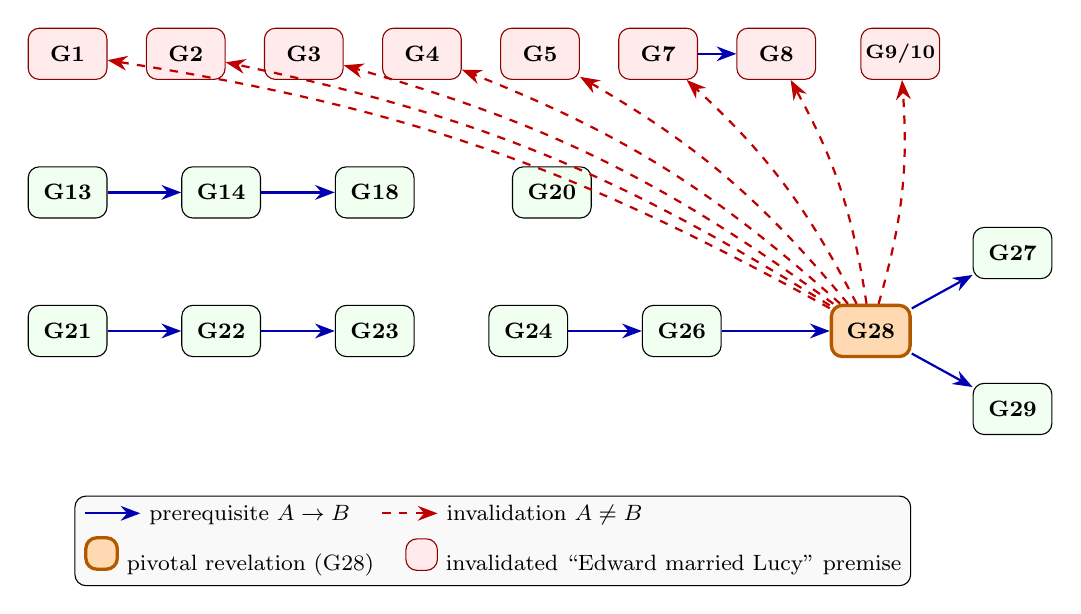
\begin{tikzpicture}[
    >={Stealth[length=2.5mm]},
    x=15mm, y=11mm,
    nnode/.style={draw,rounded corners,minimum width=10mm,minimum height=6.5mm,
                  inner sep=1pt,font=\footnotesize\bfseries,fill=green!6},
    pivot/.style={nnode,fill=orange!30,draw=orange!70!black,very thick},
    falsey/.style={nnode,fill=red!8,draw=red!55!black},
    prereq/.style={->,blue!70!black,thick},
    invalid/.style={->,red!75!black,dashed,thick},
  ]

  % --- top row: invalidated "Edward married Lucy" premises (incl. G5) ---
  \node[falsey] (g1)  at (0,4)  {G1};
  \node[falsey] (g2)  at (1,4)  {G2};
  \node[falsey] (g3)  at (2,4)  {G3};
  \node[falsey] (g4)  at (3,4)  {G4};
  \node[falsey] (g5)  at (4,4)  {G5};
  \node[falsey] (g7)  at (5,4)  {G7};
  \node[falsey] (g8)  at (6,4)  {G8};
  \node[falsey] (g910) at (7.05,4) {\scriptsize G9/10};

  % --- supposition chain ---
  \draw[prereq] (g7) -- (g8);

  % --- arrival sub-chain ---
  \node[nnode] (g13) at (0,2.4)   {G13};
  \node[nnode] (g14) at (1.3,2.4) {G14};
  \node[nnode] (g18) at (2.6,2.4) {G18};
  \draw[prereq] (g13) -- (g14);
  \draw[prereq] (g14) -- (g18);

  % --- retreat ---
  \node[nnode] (g20) at (4.1,2.4) {G20};

  % --- dialogue / discovery chain ---
  \node[nnode] (g21) at (0,0.8)   {G21};
  \node[nnode] (g22) at (1.3,0.8) {G22};
  \node[nnode] (g23) at (2.6,0.8) {G23};
  \node[nnode] (g24) at (3.9,0.8) {G24};
  \node[nnode] (g26) at (5.2,0.8) {G26};
  \draw[prereq] (g21) -- (g22);
  \draw[prereq] (g22) -- (g23);
  \draw[prereq] (g24) -- (g26);

  % --- pivot + consequences ---
  \node[pivot] (g28) at (6.8,0.8)  {G28};
  \node[nnode] (g27) at (8.0,1.7)  {G27};
  \node[nnode] (g29) at (8.0,-0.1) {G29};
  \draw[prereq] (g26) -- (g28);
  \draw[prereq] (g28) -- (g27);
  \draw[prereq] (g28) -- (g29);

  % --- invalidation fan from the pivot ---
  \foreach \t in {g1,g2,g3,g4,g5,g7,g8,g910} {
    \draw[invalid] (g28) to[bend right=10] (\t);
  }

  % --- legend ---
  \node[draw,fill=gray!5,rounded corners,anchor=north,align=left,
        font=\footnotesize] at (3.6,-1.1) {
    \tikz\draw[prereq](0,0)--(7mm,0);~prerequisite $A\rightarrow B$
    \quad
    \tikz\draw[invalid](0,0)--(7mm,0);~invalidation $A\neq B$\\[3pt]
    \tikz\node[pivot,minimum width=4mm,minimum height=4mm]{};~pivotal revelation (G28)
    \quad
    \tikz\node[falsey,minimum width=4mm,minimum height=4mm]{};~invalidated ``Edward married Lucy'' premise
  };

\end{tikzpicture}
\caption{Ground-truth dependency graph (units G1--G31). The pivot \textbf{G28}
mirrors the predicted pivot F27 (Table~\ref{tab:gt-align}); its invalidation fan
covers the same premise set, plus the ground-truth-only unit G5 (married before
ordination).}
\label{fig:gt-graph}
\end{figure}

\subsection*{Temporal-order discrepancies}

The ground-truth units \textbf{G1--G31 are listed in chronological order}: G$i$
happens before G$j$ whenever $i<j$. The altered passage, however, narrates the
\emph{same} events in a different order. Using the alignment of
Table~\ref{tab:gt-align}, we assign each predicted unit its
\emph{chronological rank} (the index of the ground-truth event it reports) and
ask whether reading F1, F2, \dots, F33 in order visits those ranks in increasing
order. Wherever a later predicted unit reports an \emph{earlier} event than one
before it, the narration has jumped backwards in time --- a temporal
discrepancy.

\paragraph{Chronological rank of each predicted unit.}
\begin{center}\small
\begin{tabular}{l*{17}{c}}
\hline
F  & 1&2&3&4&5&6&7&8&9&10&11&12&13&14&15&16&17\\
rank (G) & 10&6&11&2&3&13&14&4&\textbf{1}&7&8&18&15&9&20&20&16\\
\hline
F  & 18&19&20&21&22&23&24&25&26&27&28&29&30&31&32&33&\\
rank (G) & 19&19&\textbf{12}&21&22&23&24&25&26&\textbf{28}&\textbf{27}&29&29&30&30&31&\\
\hline
\end{tabular}
\end{center}

In a perfectly ordered paraphrase this rank sequence would be non-decreasing.
Instead it lurches: it opens at rank~10, drops to rank~2 (F4), reaches back to
rank~\textbf{1} at F9 (the chronological \emph{start} of the scene, narrated
ninth), and only settles into order from F21 onward. Two discrepancies survive
into the otherwise-ordered tail: F20 (rank~12, the missing word from Brandon,
displaced very late) and the climactic local swap F27/F28
(rank~28 before rank~27).

\paragraph{What is out of place.}
\begin{itemize}[leftmargin=*]
  \item \textbf{Scrambled opening cluster (F1--F14).} Chronologically the scene
        runs G1\,(mulls)$\to$G2\,(hoped to prevent)$\to$G3\,(hurt)$\to$
        G4\,(so soon)$\to$G6\,(Barton)$\to$G7/8\,(Delaford)$\to$
        G9/10\,(London / no letter)$\to$G11\,(asks mother)$\to$G12\,(no word).
        The paraphrase instead \emph{opens} with the missing-letter surprise
        (F1$=$G10) and the Barton musing (F2$=$G6), asks the mother (F3$=$G11)
        \emph{before} establishing the hurt (F4/F5$=$G2/G3), and reaches the true
        starting beat ``Elinor mulls over the marriage'' (F9$=$G1) only ninth.
  \item \textbf{Displaced ``no word from Brandon'' (F20$=$G12).} In the ground
        truth this immediately follows the request to write (G11); the paraphrase
        moves it past the arrival and greeting, to just before Mrs.~Dashwood's
        question about Mrs.~Ferrars.
  \item \textbf{Climactic swap (F27$\leftrightarrow$F28, i.e.\ G28 before G27).}
        The paraphrase states the revelation (Robert married Lucy) and then
        reports the general shock; the ground truth has the shocked
        ``what's the meaning of this?'' (G27) precede the explanatory reveal
        (G28).
\end{itemize}

\paragraph{Discrepancy plot.}
Figure~\ref{fig:order} plots each predicted unit at $(\text{appearance order},
\text{chronological rank})$. A faithful retelling would lie on the rising dotted
diagonal; every point \emph{below} that diagonal is an event told later than its
true time, and every \textbf{red back-arc} connects consecutive units where the
story jumps backwards in time. The dense tangle of back-arcs over F1--F14 is the
scrambled opening; the lone late arcs are F20 and the F27/F28 swap.

\begin{figure}[h]
\centering
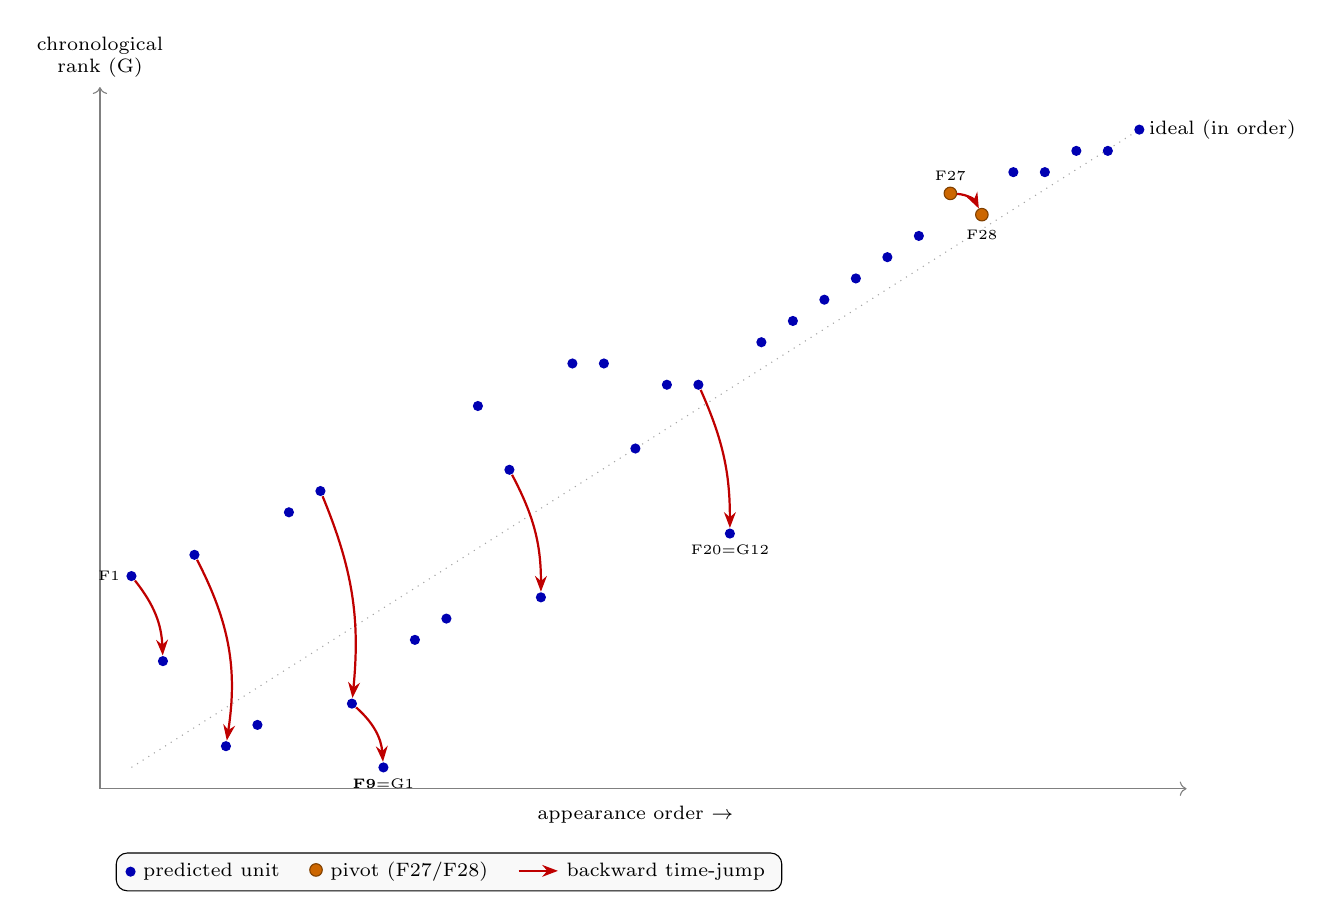
\begin{tikzpicture}[
    x=4.0mm, y=2.7mm,
    dot/.style={circle,fill=blue!70!black,inner sep=1.3pt},
    pdot/.style={circle,fill=orange!80!black,draw=orange!50!black,inner sep=1.6pt},
    back/.style={->,red!75!black,thick,>={Stealth[length=2mm]}},
    lbl/.style={font=\tiny,inner sep=1pt},
  ]

  % axes
  \draw[->,gray] (0,0) -- (34.5,0);
  \node[font=\scriptsize,below=1mm] at (17,0) {appearance order $\rightarrow$};
  \draw[->,gray] (0,0) -- (0,33) node[above,font=\scriptsize,black,align=center] {chronological\\rank (G)};
  % ideal diagonal: rank == position would be perfect; scale 31 ranks over 33 slots
  \draw[dotted,gray!70] (1,1) -- (33,31) node[right,font=\scriptsize,black] {ideal (in order)};

  % data: (Findex, chronoRank); pivot F27/F28 in orange
  \foreach \i/\r in {1/10,2/6,3/11,4/2,5/3,6/13,7/14,8/4,9/1,10/7,11/8,
                     12/18,13/15,14/9,15/20,16/20,17/16,18/19,19/19,20/12,
                     21/21,22/22,23/23,24/24,25/25,26/26,29/29,30/29,
                     31/30,32/30,33/31}
    \node[dot] (p\i) at (\i,\r) {};
  \node[pdot] (p27) at (27,28) {};
  \node[pdot] (p28) at (28,27) {};

  % label a few salient points
  \node[lbl,below=1pt of p9]  {\textbf{F9}=G1};
  \node[lbl,left=1pt of p1]   {F1};
  \node[lbl,below=1pt of p20] {F20=G12};
  \node[lbl,above=1pt of p27] {F27};
  \node[lbl,below=2pt of p28] {F28};

  % red back-arcs: consecutive F where chronological rank decreases
  % opening scramble
  \draw[back] (p1) to[bend left=18] (p2);    % 10 -> 6
  \draw[back] (p3) to[bend left=18] (p4);    % 11 -> 2
  \draw[back] (p7) to[bend left=14] (p8);    % 14 -> 4
  \draw[back] (p8) to[bend left=22] (p9);    % 4  -> 1
  \draw[back] (p13) to[bend left=14] (p14);  % 15 -> 9
  % late displacements
  \draw[back] (p19) to[bend left=12] (p20);  % 19 -> 12
  \draw[back] (p27) to[bend left=30] (p28);  % 28 -> 27 (climactic swap)

  % legend
  \node[draw,fill=gray!5,rounded corners,anchor=north west,align=left,
        font=\scriptsize] at (0.5,-3) {
    \tikz\node[dot]{}; predicted unit \quad
    \tikz\node[pdot]{}; pivot (F27/F28) \quad
    \tikz\draw[back](0,0)--(5mm,0); backward time-jump
  };

\end{tikzpicture}
\caption{Temporal-order discrepancy plot. Each predicted unit F$i$ is placed at
its appearance order ($x$) and the chronological rank of the ground-truth event
it reports ($y$). A faithful retelling tracks the dotted diagonal; points below
it are told late, and red arcs mark consecutive backward jumps in time. The
opening cluster F1--F14 is badly scrambled (it reaches the true first event,
F9$=$G1, only ninth), while F21--F33 is ordered apart from the displaced F20 and
the climactic F27/F28 swap.}
\label{fig:order}
\end{figure}

\end{document}
